\section{Modélisation conceptuelle}\label{sec:concept}
% \e{}
% On divise notre problème de modélisation en axes 
% comme il n'existe pas UNE prod.av, on propose des briques représentant des situations typiques paramétrables pour s'ajuster à un usage particulier
% on présente le concept principal, la structure ontologique, les articulations avec le reste de l'ontologie, et un exemple d'utilisation

Comme nous l'avons vu en section \ref{sec:metier}, la production audiovisuelle suit une structure générale qui peut être amenée à changer dans le cadre de productions collaboratives mobilisant des objets existants (\ref{sec:rechaine}) ou bien en fonction du type de production (\ref{sec:strat-desc}).
Ainsi, il apparaît que \gui{\pc{la} production audiovisuelle} n'existent pas, mais recouvrent un ensemble de pratiques et d'usages.
Néanmoins, il existe une tradition de travail et d'organisation de la production en projet, lui-même décomposé en grandes étapes (pré-production, production, post-production) et articulés autour de rôles phares (réalisateur, acteur, chef-opérateur, preneur de son etc.) dont les responsabilités sont, là encore, relativement définies, mais sujettes aux changements suivant la nature de la production, de l'organisation, de traditions nationales etc.

Notre modélisation vise donc à fournir des briques de bases pour représenter l'organisation d'un projet de production.
En suivant la synthèse de scénario de la section \ref{sec:scenar-apps}, cela correspond à l'étape (2) de \g{Planification} qui sera susceptible d'être modifié tout au long de la chaîne, suivant les péripéties de son déroulement.
Cette approche générique permet à chacun de définir sa propre hiérarchie de tâches et de distribuer finement les responsabilités entre les différents contributeurs du projet.


\subsection{Axes de modélisation}
Notre travail de modélisation se heurte à deux verrous scientifiques, identifiés en section \ref{sec:scien} puis développé dans les chapitre \ref{chap:omod} et \ref{chap:mav}, que nous reformulons en : 


\begin{problemes}{LightGoldenrodYellow}
\begin{liste}
 	\item[(\g{$\alpha$})] \g{l'articulation de plusieurs ensembles de connaissances} [\e{$\chi_1$ : autonomie}, \e{$\chi_2$ : réutilisabilité}]. 
 	On distingue ainsi deux ensembles de connaissances : 
 	% à quoi servent-ils ?
 	\begin{listeni} 
 		\item[($\alpha_1$)] l'organisation du \e{processus de production audiovisuelle}, qui décrit la répartition des tâches et  les capacités des \e{contributeurs}.
 		Cet ensemble permet d'associer les connaissances fabriquées par les contributeurs aux documents et de faciliter leur implication et les échanges de connaissances.
 		
 		\item[($\alpha_2$)] l'organisation du \e{document audiovisuel}, c'est-à-dire sa structure documentaire, le \e{matériel audiovisuel} qu'on y attache et une description de leur fabrication (l'\e{écriture filmique} détaillée dans le script).
 		Cet ensemble permet de faciliter la recherche, la gestion et donc la réutilisation des fragments audiovisuels.
 	\end{listeni}

 	\item[(\g{$\alpha$})] et \g{une pro(duction/con)sommation progressive et contributive de ces connaissances} [\e{$\delta_1$: multi-jargon}, \e{$\delta_2$ : documentation}, \e{$\delta_3$ : évolution, gestion}].
 	Il s'agit ici du problème de l'évolution et du partage des connaissances liées à un document/fragment audiovisuel tout au long de son ou de ses cycle(s) de vie. 
 	On distingue deux écueils nouveaux suite à l'ouverture de la chaîne à des pratiques de réutilisation : la \e{progressivité de la description}, et la nécesssité de la rendre compréhensible malgré l'\e{hétérogénéité des contributeurs} : 
 	\begin{listeni}
 		\item[($\beta_1$)] \e{les connaissances sur les document/fragments audiovisuels évoluent et s'ajustent au contexte de production ou de réutilisation}.
 		Les connaissances fabriquées en début de chaîne de production prescrivent un résultat attendu, or de nombeux éléments sont susceptibles d'être modifiés ou précisés par la suite.
 		Il faut donc ajuster les connaissances prescriptives à la réalité des opérations, afin de décrire les résultats effectifs (et non plus l'attendu).
 		Cet écueil apparent est en réalité une opportunité, car la fabrication des descriptions peut alors s'appuyer sur les connaissances prescriptives et les vérifier. 
		De plus, la réutilisation d'un fragment/document audiovisuel dans un nouveau contexte n'implique pas seulement un transfert de matériels audiovisuels, mais également un transfert des connaissances. % mais est-ce que l'on traite vraiment ce cas ? on gère des ensembles de connaissances qui peuvent évoluer (enrichissement)
		Ce transfert peut nécessiter d'extraire certaines connaissances toujours pertinentes et de les associer à celles du nouveau contexte d'utilisation, ou bien de les intégrer à une conceptualisation propre à ce contexte (spécialisation ou bien extension).
		% Cette évolution est rendue possible par 

		\item[($\beta_2$)] \e{adapter la forme d'expression des connaissances en fonction de l'implication du contributeur dans la chaîne de production et de ses capacités.}
 		Le problème de l'accès aux connaissances est traité par la composition d'une vue contextuelle et spécifique à chaque contributeur de la chaîne, ou chaque groupe de contributeurs.
 		Toute connaissance exprimée à travers le modèle doit pouvoir être caractérisée suivant les codes d'écritures utilisés, eux-mêmes reliées aux capacités des contributeurs.
		Il est alors possible d'effectuer une double sélection ; les connaissances pertinentes suivant l'implication dans la chaîne (en utilisant la description du processus de production); les formes d'expression facilitant leur compréhension (à partir d'une description des capacités des contributeurs).
		% Cette adaptation est rendue possible par le couplage entre conceptualisation, terminologie et documentation.
 	\end{listeni}
\end{liste}
\end{problemes}

% (\ref{sec:cdc-av}). 



% Par ailleurs, les objectifs métiers de réutilisation ouvre la chaîne de production à de nouveaux contributeurs, dont les niveaux de compétences et de compréhension sont variables (\ref{sec:cdcf}). 
% Les connaissances liées à la production doivent être rendues accessibles à toutes les contributeurs de la chaîne, de même qu'ils doivent contribuer à la fabrication de ces connaissances, tout autant que la fabrication d'objets audiovisuels ou de documents métiers. 

% L'approche que nous avons suivi se positionne sur deux axes de modélisation : 
% \begin{liste}
% 	\item[\g{$\alpha$}] articuler une modélisation conceptuelle aux problèmes de partage et de construction de connaissances communes d'une chaîne de production audiovisuelle ouverte et hétérogène. 
% 	Nous traitons dans cet axe les problèmes définis dans le chapitre \ref{chap:omod} sur la nécessité de construire des terminologies multi-jargon [\g{A1}], d'enrichir une conceptualisation avec de la documentation [\g{A2}], et de gérer l'évolution des unes et des autres de manière indépendantes [\g{A3}].



Relations transitives pour faciliter l'inférence (SKOS) ; distinction entre objet réel (production) et fictif (diégèse) (DMS-1).


\subsection{Situations typiques des productions audiovisuelles}
Notre modélisation peut se décomposer en situations typiques qui se retrouvent dans tous les types de productions audiovisuelles.
Nous présentons ces situations en rapport avec les axes de modélisations que nous avons défini :
\begin{listeni}
	\item[($\alpha_1$)] l'organisation du \g{processus de production} et du travail de ses \g{contributeurs} : 
	\begin{liste}
		\item la division d'un projet de production en sous-tâches et la spécification du résultat attendu ainsi que des moyens fournis pour les remplir.

		\item l'assignation des tâches d'un projet à des contributeurs, ce qui leur confère un rôle, des droits et des responsabilités.
	\end{liste}

	\item[($\alpha_2$)] l'articulation d'un \g{document audiovisuel} et de ses différentes composantes, avec leurs descriptions : 
	\begin{liste}
		\item la structure documentaire qui suit des règles de composition de fragments.
		\item la segmentation du matériel audiovisuel.
		\item la gestion des fichiers qui encapsulent le matériel audio-visuel et ces différentes pistes.
		\item la description par l'écriture filmique, et ses références à des éléments fictifs ou réels.
	\end{liste}


	\item[($\beta_1$)] le déroulement de la production a pour conséquence de faire \g{évoluer nos connaissances} sur l'organisation du processus de production et l'articulation du document audiovisuel : 
	\begin{liste}
		\item les pratiques de réutilisation de fragments documentaires.
		\item l'évolution de la description d'un document audiovisuel.
		\item l'échange de connaissances entre organisations.
	\end{liste}

	\item[($\beta_2$)] l'\g{adaptation des formes d'expressions} aux capacités des contributeurs de la chaîne de production : 
	\begin{liste}
		\item l'attribution de compétences linguistiques et professionnelles aux contributeurs (humains, machines).
		\item la mise en place d'un thésaurus multi-jargon et d'une documentation des concepts.
		\item l'accès personnalisé aux connaissances de la chaîne suivant le contexte (le contributeur, ses capacités, son implication dans la châine).
	\end{liste}

\end{listeni}



%%%%%%%%%%%%%%%%%%%%%%%%%%%%%%%%%%%%%%
\subsubsection{Articulation des composants d'un document audiovisuel}
\paragraph{Structure ontologique}
\paragraph{Relations avec d'autres concepts}

%%%%%%%%%%%%%%%%%%%%%%%%%%%%%%%%%%%%%%
\subsubsection{Description par l'écriture filmique}
\paragraph{Structure ontologique}
\paragraph{Relations avec d'autres concepts}

%%%%%%%%%%%%%%%%%%%%%%%%%%%%%%%%%%%%%%
\subsubsection{Hiérarchie des tâches dans un projet de production}
La définition d'une hiérarchie de tâches repose sur la définition d'une unité de travail représenté par le concept de \con{Mission} : 

\begin{cadrecol}{LightGoldenrodYellow}
Une \con{Mission} représente un ensemble d'actions cohérentes, réalisées de manière intentionnelles afin de mener à bien un processus de production. 
Ces actions peuvent être exécutées par un ou plusieurs contributeurs, réutilisant parfois des objets existants (ressource), et aboutir à la gestion du processus de production (\con{Mission} de gestion ou de validation : \con{Project} et \con{Activity}), ou bien à la fabrication d'un résultat attendu (ou livrable, pour les \con{Mission}s de fabrication : \con{Task}). 
Par exemple, une \con{Mission} de tournage peut être réalisée par un caméraman, ou bien une équipe de tournage et aboutit à la fabrication de matériel audiovisuel.
\end{cadrecol}

 

\paragraph{Structure ontologique} 
La production d'un film requière de nombreux contributeurs et la spécification de nouvelles \con{Mission}s.
Ainsi, on distingue les \con{Mission}s (dites de gestion) qui consistent à en définir d'autres, à suivre leur déroulement et à valider le résultat fabriqué par les \con{Mission}s de fabrication. 
Nous distinguons trois types de \con{Mission} par leur nature et leur importance en terme de durée : 
\begin{liste}
	\item un \con{Project} représente un projet de production, qui renvoit à entité administrative auquelle une organisation transfère des ressources (humaines, financières, équipements etc.) pour accomplir des objectifs. 
	Il s'agit d'une \con{Mission} de gestion qui ne fabrique rien, mais dirige, organise et délégue le travail et les ressources à d'autres \con{Mission}s (\con{Activity} et \con{Task}).
	Par exemple, le \con{Project} Magazine\#48 représente le processus de création de l'épisode 48 d'un programme d'information (résultat), qui consiste à commenter des évènements culturels de l'année dernière (ressource).

	\item une \con{Activity} est une étape ou un jalon d'un projet de production. 
	C'est une \con{Mission} de gestion qui consiste à organiser une séquence de \con{Task}s.
	Par exemple, une \con{Activity} nommée Post-Production peut regrouper toutes les \con{Task}s montage, retouches, effets spéciaux, post-traitements etc.

	\item une \con{Task} est une \con{Mission} opérationnelle qui vise généralement à fabriquer ou manipuler un objet audiovisuel ou des connaissances associées.
	Par exemple, le tournage d'une interview ou bien la transformation du scénario en script de tournage. 
\end{liste}

\begin{figure}[ht!]
\centering
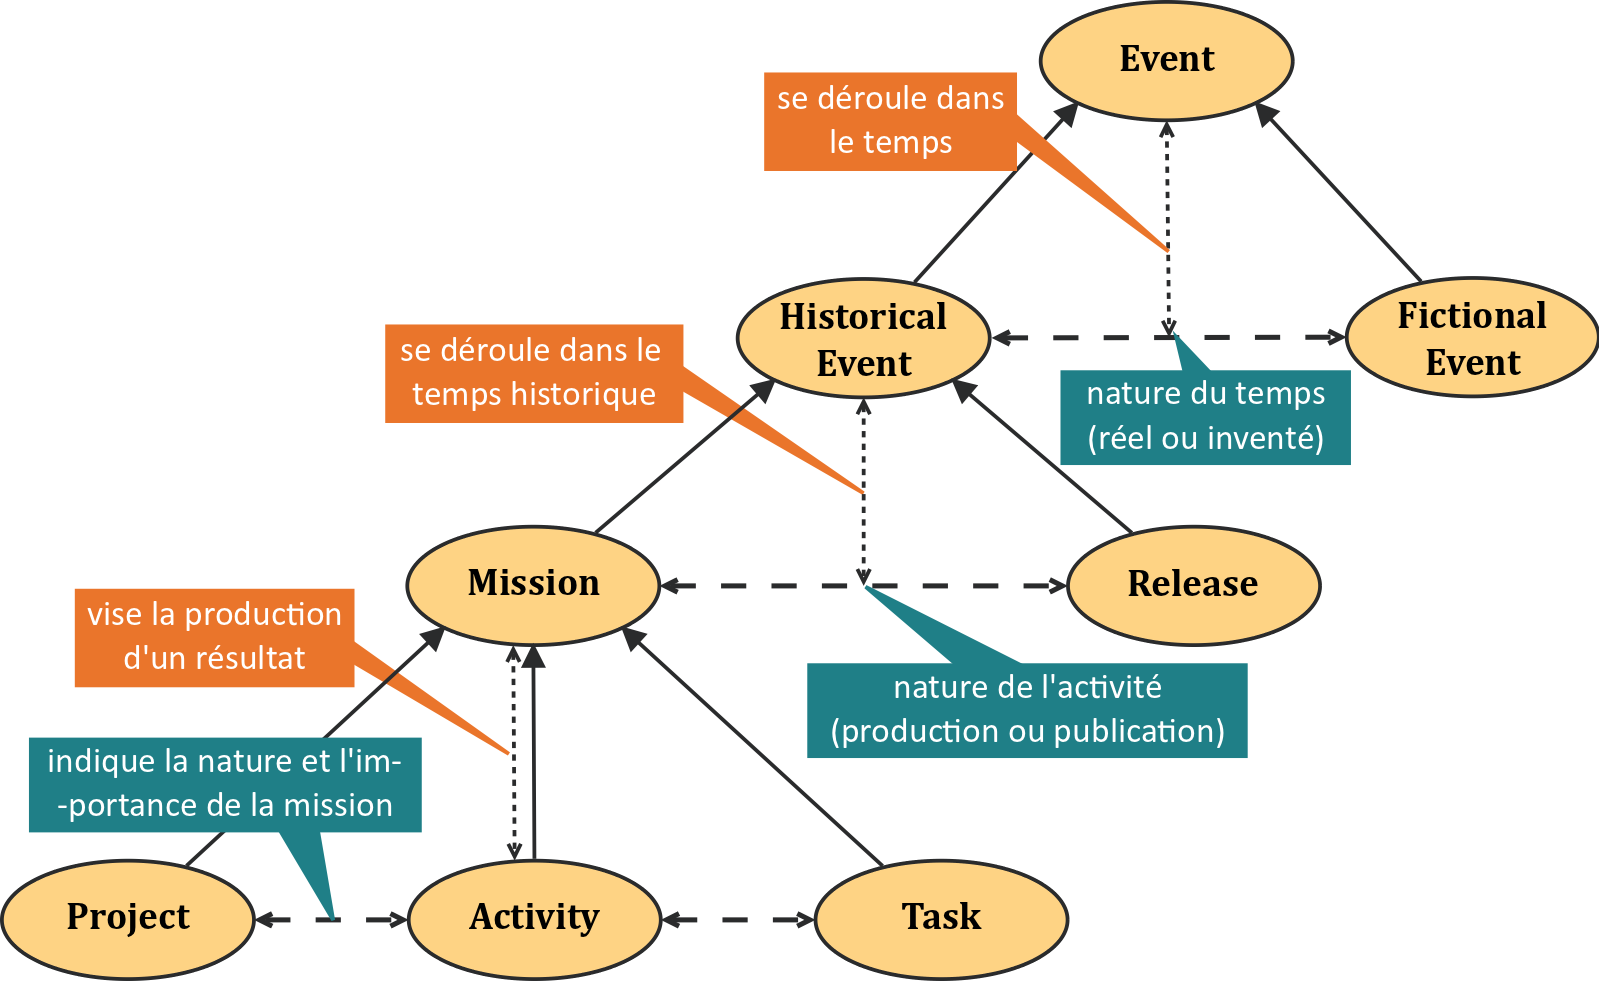
\includegraphics[width=0.95\textwidth]{./images/SO-Event-v1.png}
\caption{Extrait de la structure ontologique des évènements et de la hiérarchie des tâches d'un projet de production}
\label{img:so-event}
\end{figure}


La Figure \ref{img:so-event} précise la structure ontologique des évènements et en particulier la hiérarchie des tâches d'un projet de production.
Un point important à noter est que notre modélisation ne distingue pas les objets temporels duratifs et ponctuels, mais laisse libre choix de préciser le moment de début et de fin d'un \con{Event} à travers les propriétés \rel{Start} et \rel{End}.
Au lieu de cela, nous distinguons les évènements réels (\con{HistoricalEvent}) des évènements fictifs (\con{FictionalEvent}), qui sont mis en scène pour être filmé. 
Cette distinction se retrouve dans d'autres parties de notre modélisation et apparaît importante pour distinguer les connaissances liées à la production de celles liées à l'univers filmé (contrairement à la confusion qui existe dans DMS-1, voir \ref{sec:dms-1}).



\paragraph{Relations avec d'autres concepts}
Le concept d'\con{Event} et de \con{Mission} se définissent également par leurs relations avec le reste de notre ontologie, voir la Figure \ref{img:cr-event}. 
Voici les relations qui s'appliquent à tous les évènements : 
\begin{liste}
	\item Il est possible de spécifier la participation d'une personne ou d'une organisation (\con{Agent}) à l'évènement (par la relation \rel{hasParticipant}/\rel{isAParticipantOf}).
	Cette relation présente une version simplifiée de notre modélisation de l'implication d'un contributeur dans un projet de production.
	Nous ajoutons également une contrainte de cohérence : dans le cas où il s'agit d'évènement réel, seul des participants réels peuvent être associées à l'évènement (et inversement). 
	Par exemple, Batman ne peut pas participer à une manifestation sur la place de la Bastille, par contre Benjamin Diemert si. 

	\item Il est possible de localiser (\con{Location}) l'évènement (par la relation \rel{isLocatedIn}).
	Cette relation en fonctionne que dans un seul sens et ne peut pointer que vers un lieu, qui lui-même est liée à d'autres lieux par des relations méréologiques ou d'autres relations géographiques.
	Nous ajoutons également une contrainte de cohérence : un évènement réel ne peut se situer dans un lieu fictif.

	\item Les évènements peuvent également être le sujet d'une oeuvre (\con{Opus}) grâce à la relation \rel{isATopicOf}. 
\end{liste}


\begin{figure}[ht!]
\centering
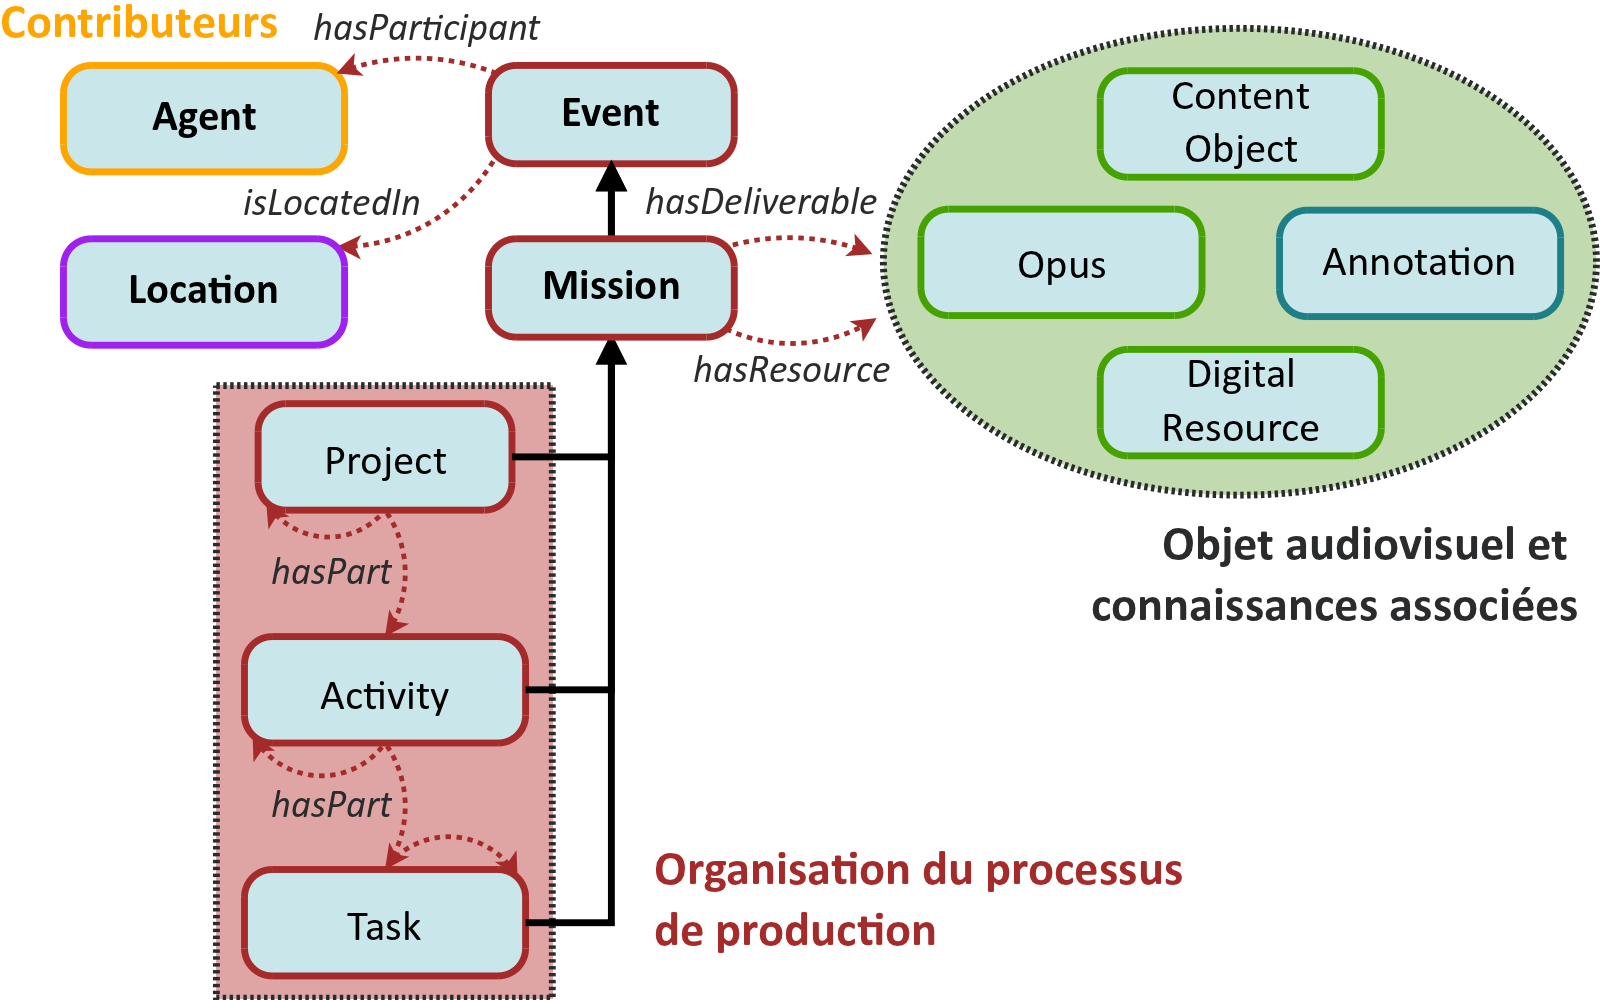
\includegraphics[width=0.75\textwidth]{./images/MOD-Process-v2.png}
\caption{Principaux concepts et relations pour la modélisation d'une hiérarchie de tâches}
\label{img:cr-event}
\end{figure}


À cela, s'ajoute les relations qui s'appliquent spécifiquement aux \con{Mission}s : 
\begin{liste}
	\item Il est possible de spécifier un ou plusieurs résultats attendus (ou livrable) pour chaque \con{Mission} (relation \rel{hasDeliverable}/\rel{isADeliverableOf}).
	Ce livrable peut être soit un document ou fragment audiovisuel (\con{Opus}), une séquence de matériel audiovisuel (\con{ContentObject}), un fichier (\con{DigitalResource}) ou bien une description (\con{Annotation}).
	Par exemple, une \con{Task} de tournage vise à produire une séquence audiovisuelle alors qu'une \con{Task} de transcodage vise à produire un nouveau fichier vidéo.

	\item Il est possible d'associer un ou plusieurs éléments existants (ou ressource) à chaque \con{Mission} (\rel{hasResource}/\rel{isAResourceFor}). 
	Cette ressource peut être soit un document ou fragment audiovisuel (\con{Opus}), une séquence de matériel audiovisuel (\con{ContentObject}), un fichier (\con{DigitalResource}) ou bien une description (\con{Annotation}).
	Par exemple, le \con{Project} Magazine\#48 utilise des séquences audiovisuelles (\con{Segment}) tournées l'année dernière.

	\item Il est possible d'indiquer un ordre de réalisation des \con{Mission}s grâce à des relations d'anteriorités (\rel{precedes}, \rel{precedesTransitive}) et de postériorités (\rel{follows}, \rel{followsTransitive}).
	Les propriétés transitives généralisent les autres propriétés afin de faciliter le raisonnement par inférence (à la manière de SKOS, \ref{sec:skos}).

	\item Il est possible de spécifier des relations hiérarchiques entre les types de \con{Mission}s par la relation \rel{hasPartTransitive}/\rel{isPartOfTransitive} et \rel{hasPart}/\rel{isPartOf}.
	Nous ajoutons des restrictions afin que chaque type de Mission ne puisse englober que des Missions du même type, ou bien de niveau inférieur, de manière à créer des niveaux . 
	Ainsi, un Project peut tout englober, mais une Task ne peut s'englober qu'elle-même. 
	Inversement, une Task peut être englobée dans tous types de Mission, mais un Project ne peut qu'être englobé par lui-même.
\end{liste}





%%%%%%%%%%%%%%%%%%%%%%%%%%%%%%%%%%%%%%
\subsubsection{Les contributeurs et leur engagement dans un projet de production}
Notre modélisation des contributeurs repose sur la notion d'\con{Agent} humain ou logiciel :
\begin{cadrecol}{LightGoldenrodYellow}
Un \con{Agent} représente une entité avec des capacités d'actions (contrairement à une ressource), qui peuvent être mises en oeuvre dans le cadre d'un évènement (\con{Event}).
Par exemple, l'\con{Agent} chargé d'identifier les personnes dans un plan peut être une documentaliste ou bien un logiciel de reconnaissances de visage.
\end{cadrecol}

En plus de cette notion de contributeur, il faut également modéliser la notion d'engagement, ce qui se représente classiquement par les notions de rôle et de droits.
Dans le cadre d'une modélisation des productions audiovisuelles, nous devons faciliter le paramétrage des responsabilités attribuées à chacun de ces rôles. 
Pour cela, nous introduisons la notion de poste (\con{Position}) à laquelle nous rattacherons des droits (\con{Right}s) sur les \con{Mission}s.

\begin{cadrecol}{LightGoldenrodYellow}
Un \con{Role} représente un poste générique d'un projet de production. 
L'attribution d'un rôle peut être soumise à la reconnaissance des compétences (\con{Skill}) du contributeur.
Par exemple, un caméraman doit avoir une compétences sur le maniement d'une caméra professionnelle.
\end{cadrecol}

\begin{cadrecol}{LightGoldenrodYellow}
Une \con{Position} représente un poste et un contexte de travail particulier.
Il s'agit de préciser quel est l'employeur du contributeur, dans quel projet de production (\con{Project}) il est impliqué ainsi que les responsabilités et les droits (\con{Right}) qu'on lui a confié. 
L'attribution d'une \con{Position} peut être soumise à la reconnaissances des compétences (\con{Skill}) du contributeur.
Par exemple, Boris est engagé en tant qu'assistant réalisateur par la RTBF dans le projet de production Magazine\#48.
Il sera chargé de réaliser les interviews hors plateau.
L'ensemble de ces informations correspond au poste de Boris.
\end{cadrecol}

Toutefois, si une \con{Position} permet de représenter les responsabilités réelles de chaque contributeur, la notion de rôle (\con{Role}), quant-à-elle, sert de repère conventionnel (auteur, réalisateur, caméraman etc.) et permet de définir des règles génériques d'attributions de droits.
Par exemple, un auteur sur un projet Z peut être responsable de l'écriture du scénario et de la continuité (ajout des dialogues et détails des actions), alors que ce travail sera confié respectivement à l'auteur et au dialoguiste sur un projet Y.
On peut également écrire une règle qui attribuent des droits de validation à un producteur sur l'ensemble du projet de production, ou juste une activité.


\begin{figure}[ht!]
\centering
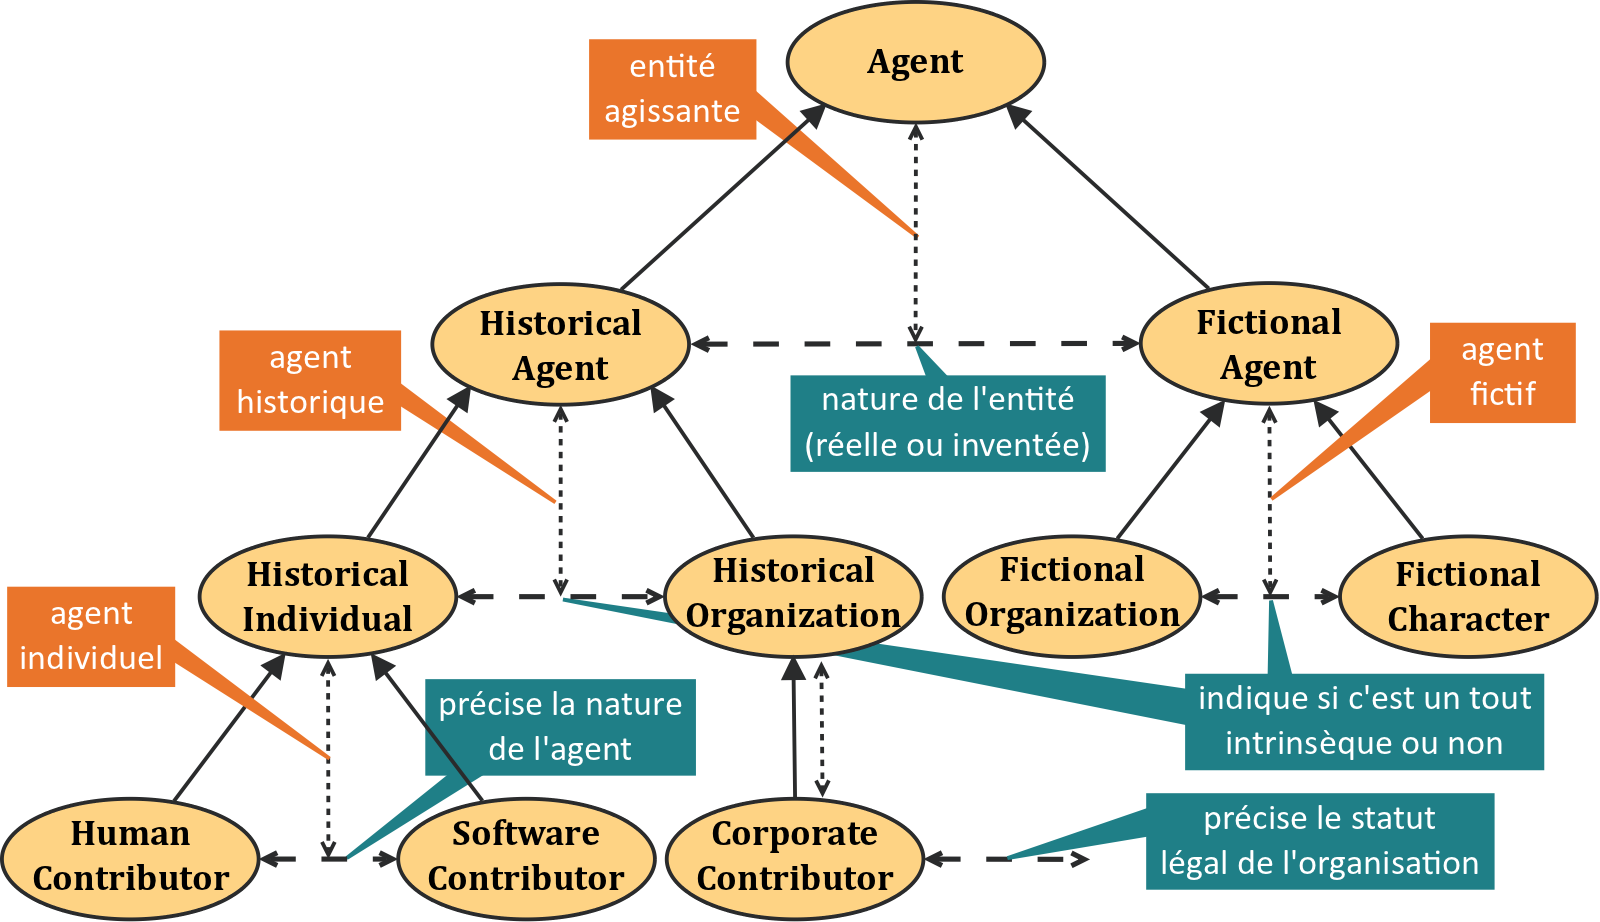
\includegraphics[width=0.95\textwidth]{./images/SO-Agent-v1.png}
\caption{Extrait de la structure ontologique des agents et des contributeurs à un projet de production}
\label{img:so-agent}
\end{figure}

\paragraph{Structure ontologique}
\paragraph{Relations avec d'autres concepts}

























% \subsection{Prise en compte du multi-jargon}\label{}

% \subsubsection{Concept et termes}\label{sec:onter}
% Le modèle concept-terme que nous avons développé étend la représentation de la terminologie à son contexte d'accès, voir \cite{Diemert2010} et \cite{Diemert2011a}. Dans un premier temps, on associe à chaque concept un ou plusieurs termes, une définition voire une illustration. Chaque terme est caractérisé par son appartenance à une ou plusieurs notations qui représentent une langue, un vocabulaire métier, un code d'écriture, etc. Les fichiers peuvent être caractérisés de manière équivalente, voir figure \ref{img:mj-ct}.


% \begin{figure}[ht!]
% \centering
% 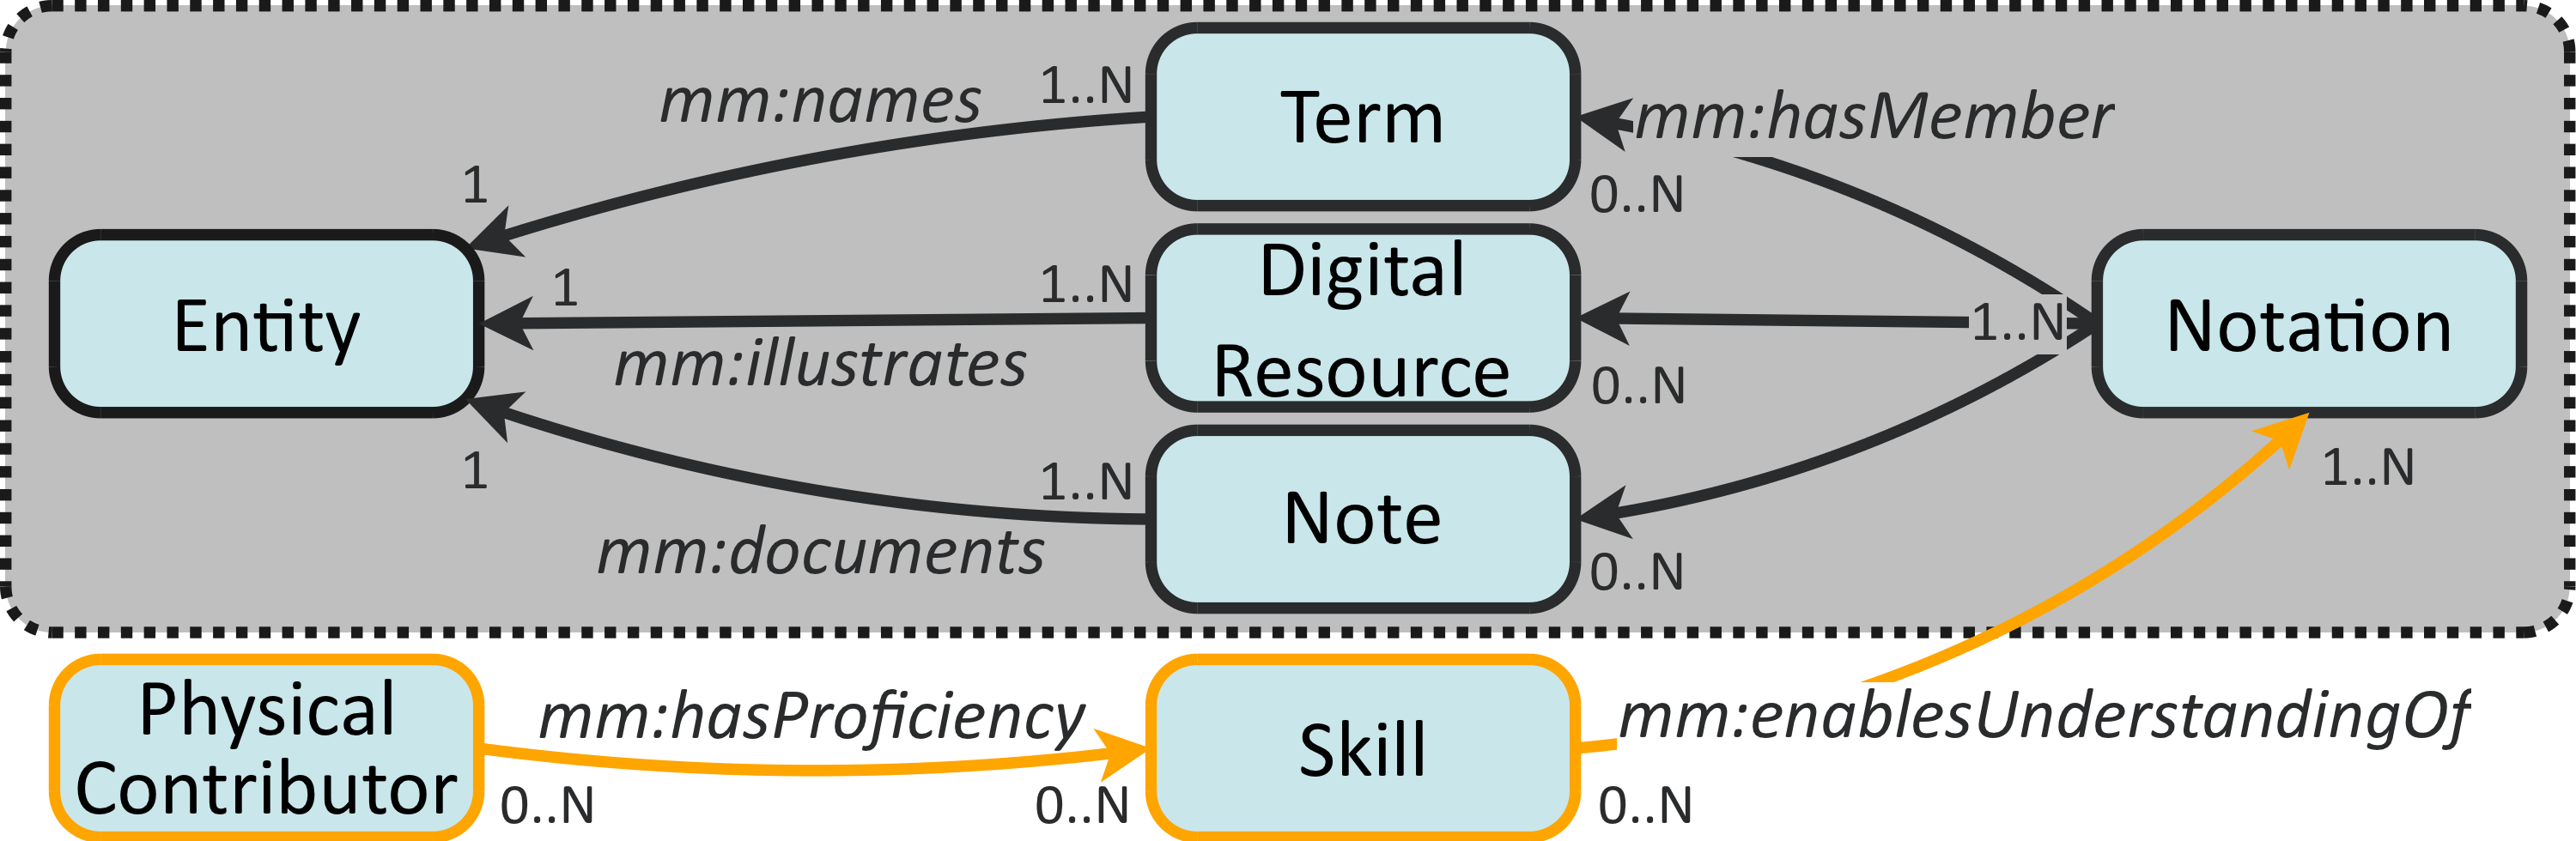
\includegraphics[width=0.75\textwidth]{./images/MOD-TermConcept-v5a.png}
% \caption{}
% \label{img:mj-ct}
% \end{figure}


% % \begin{cadrecol}{LightGoldenrodYellow}
% 	\con{Entity} représente un concept auquel on peut associer
% 		un terme (\con{Term} -- \rel{mm:names} / \rel{mm:isNamedBy}) ; une ressource média (\con{DigitalResource} -- \rel{mm:illustrates} / \rel{isIllustratedBy}) ou bien une note de documentation (\con{Note} -- \rel{mm:documents} / \rel{is\-Docu\-mentedBy}).
% % \end{cadrecol}

% % \begin{cadrecol}{LightGoldenrodYellow}
% 	\con{Term} représente un terme portant une valeur lexicale que l'on peut associer à un concept via la relation \rel{mm:names}.
% 	Un \con{Term} est caractérisé par son appartenance à un type de \con{Notation} (\rel{mm:isMemberOf} / \rel{mm:hasMember}).
% % \end{cadrecol}

% % \begin{cadrecol}{LightGoldenrodYellow}
% 	\con{Notation} représente une caractéristique commune d'un ensemble de \con{Term} ou de ressource numérique \con{DigitalResource}. 
% 	Il s'agit par exemple d'une langue, d'un format de fichier, d'un type d'encodage de date ou bien d'une structure terminologique propre à une communauté de pratiques ou une communauté d'utilisateurs.
% 	Chaque \con{Term} peut être décrit par une ou plusieurs \con{Notation}, chacune spécifiant une caractéristique particulière.
% 	Par exemple, l'étiquette \e{Plan américain} peut être décrite come appartenant à la langue française ainsi qu'à une liste d'autorité de types de plan.
% 	On distingue quatre types de \con{Notation} : 
% 	\begin{liste}
% 		\item \con{NaturalLanguage} représente les langues humaines.
% 		\item \con{SyntaxEncodingScheme} représente un codage de l'information comme l'encodage des caractères ou bien un format de fichier. 
% 		\item \con{AuthorityList} représente une liste d'autorité composé de termes. 
% 		\item \con{VocabularyEncodingScheme} (VES) représente un SOC ou un jargon propre à une organisation ou un métier.\\
% 	\end{liste}

% % \end{cadrecol}


% \paragraph{Documentation}
% % \begin{cadrecol}{LightGoldenrodYellow}
% 	\con{Note} représente une chaîne lexicale dont le but est de documenter un concept (\con{Entity}). 
% 	Nous définissons des spécialisations de \con{Note} à la manière de SKOS, par exemple pour la définition d'un concept (\con{DefinitionNote}). 
% % \end{cadrecol}

% \con{DigitalResource} représente un fichier numérique. Par exemple, un fichier texte, une photo ou bien un son. 



% \subsubsection{Conceptualisation et bases de connaissances}\label{}
% \begin{figure}[ht!]
% \centering
% 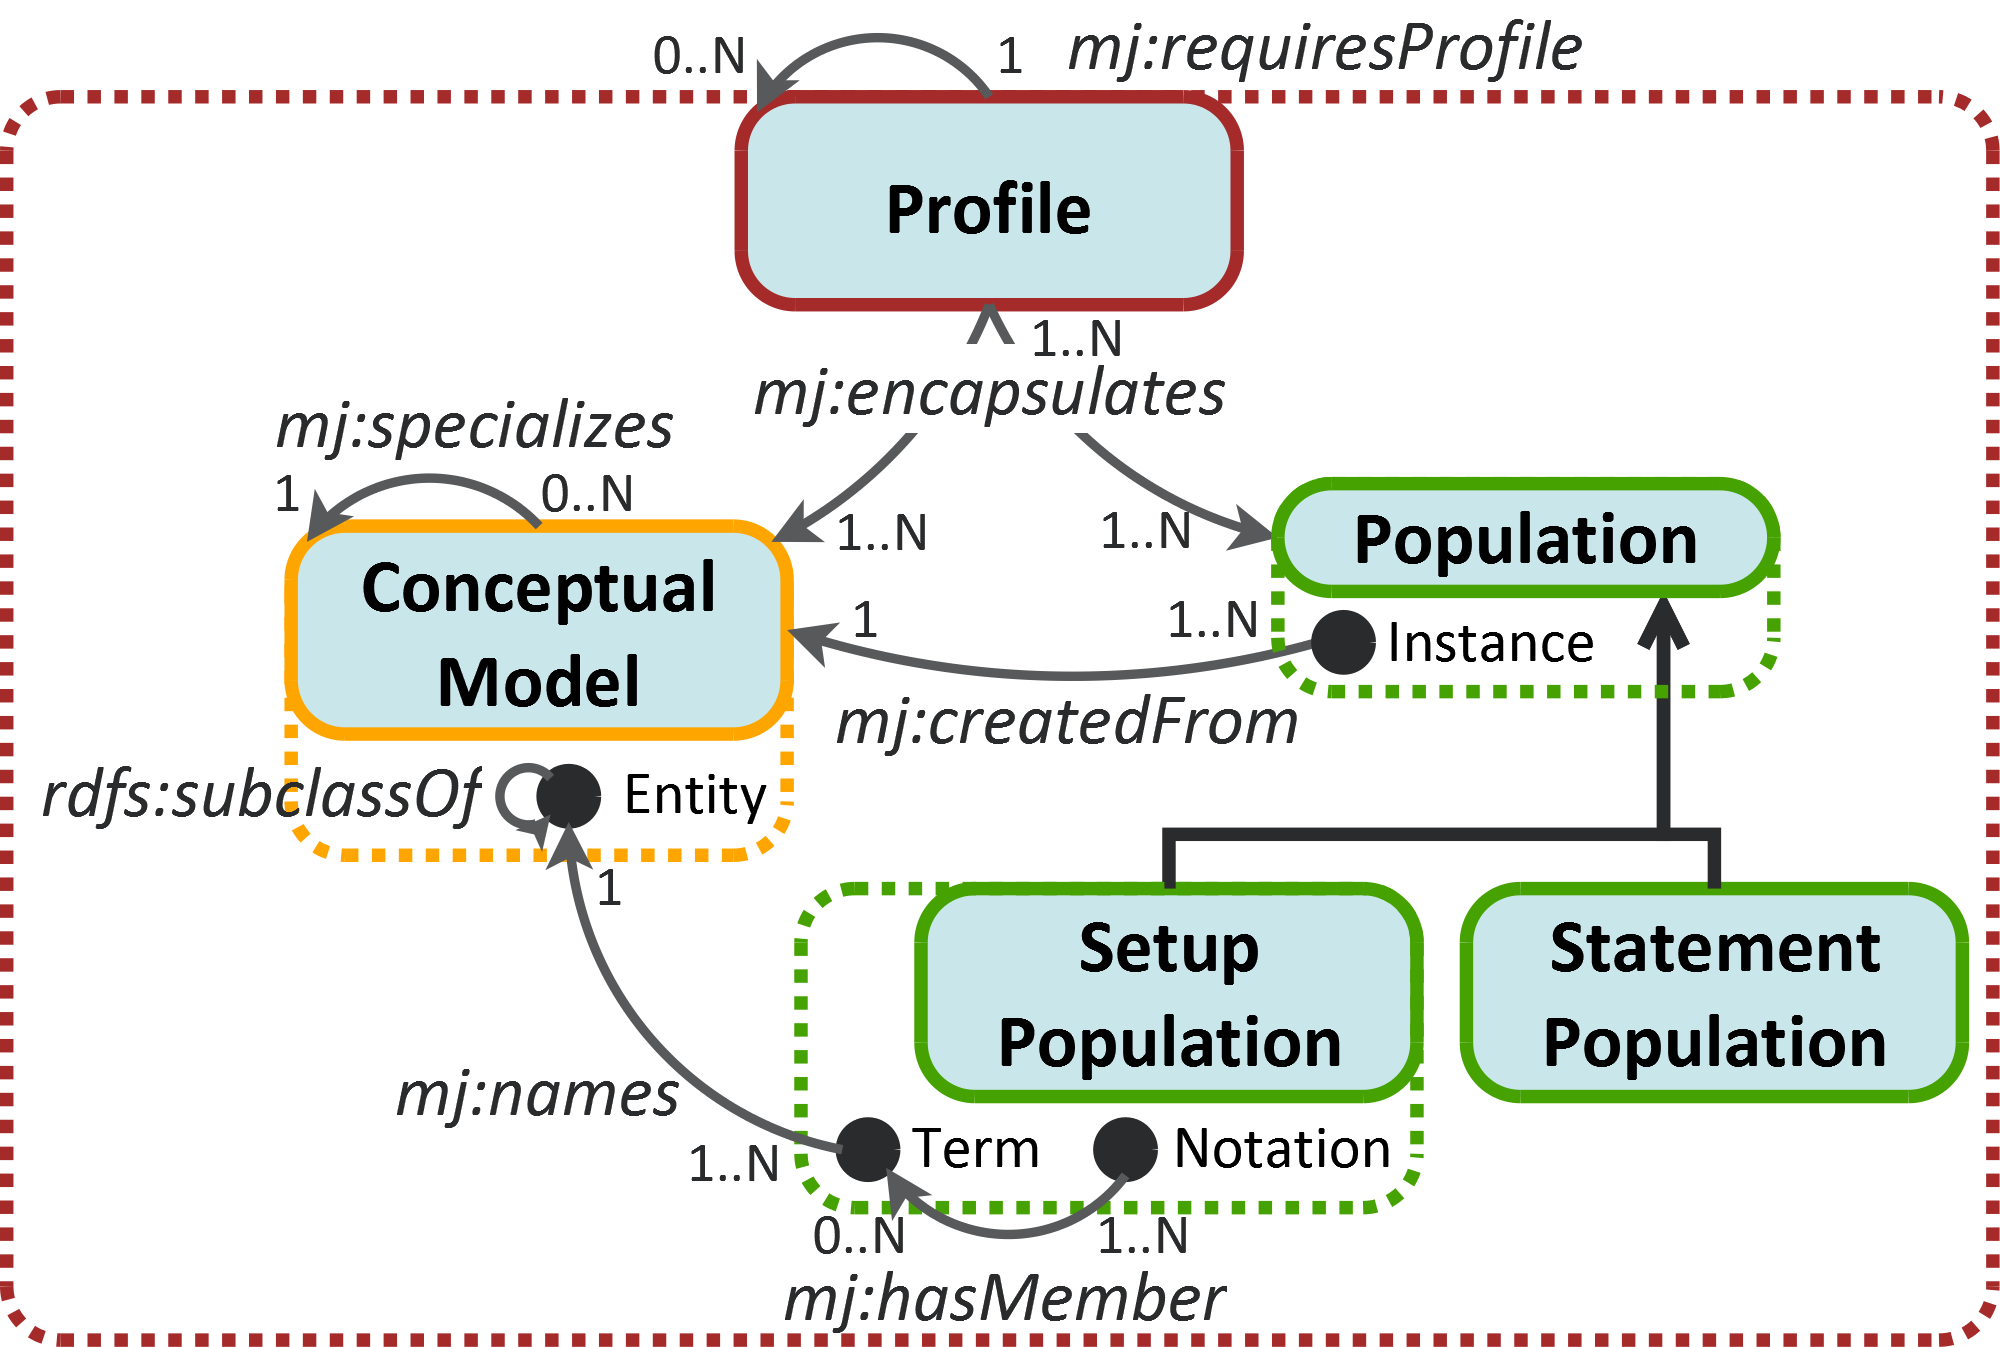
\includegraphics[width=0.7\textwidth]{./images/MOD-Profile-v3.png}
% \caption{}
% \label{img:conceptualisation}
% \end{figure}


% \subsubsection{Vue et contexte d'accès}\label{}

% % \begin{cadrecol}{LightGoldenrodYellow}
% % 	\con{} 
% % \end{cadrecol}

% \subsection{Le processus de production audiovisuelle}\label{}
% \subsubsection{Projet, Produit, Contributeur}\label{}
% \subsubsection{L'écriture filmique}\label{}


% \subsection{Le document audiovisuel}\label{}
% \subsubsection{Structure documentaire}\label{}
% \subsubsection{Manifestations}




